
%
\begin{frame}
\frametitle{}
\begin{center}
  \textbf{\Large Multi-dimensional Indexing of MOKP solutions}
\end{center}
\end{frame}

%
\begin{frame}
\frametitle{Dominance check operation}
During the process of solving a MOKP or other multi-objective problems
one of the main general operation is to check if a solution is dominated
by another. \\
\pause \bigskip
An algorithm usually requires selecting all non-dominated solutions
from a large set of partial solutions. \\
\pause \bigskip
This may demand quadratic effort on total number of solution if implemented
as pairwise comparison. \\
\pause \bigskip
However, if solutions are mapped into points in a multi-dimensional space,
this operation corresponds on checking whether a point exists in a certain region.
\end{frame}

%
\begin{frame}
\frametitle{Dominance check operation}
Formally:
\begin{align*}
    \text{ if } \; &\domk{y}{x} \; \text{ then } \; \pnt{y} \in R(\sol{x}) \\
  \text{where} \phantom{mmmmm} \\
    \pnt{x} &= \big(\obj{1}{x}, \ldots, \obj{\np}{x}, \weight{x}\big) \\
    R(\sol{x}) &= \left\{ a \in \mathbb{R}^{\np+1} \;\middle|\;
      a_{\np+1} \leq \weight{x}
      \, \text{ and } \,
      a_i \geq \obj{i}{x}, \; i \in \{1, \ldots, \np\}
      \right\}
\end{align*} \pause
\begin{figure}
  \centering
  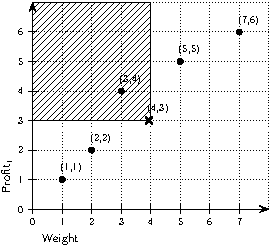
\includegraphics[scale=0.8]{img/kdt/dom}
\end{figure}
\end{frame}

%
\begin{frame}
\frametitle{Multidimensional solution indexing}
The problem of determining whether a point exists in a certain region
of space is known as \emph{range search}.
\\ \bigskip \pause
For efficiency reason range search operations is usually executed with the
assistance of a \kdtree{}.
\\ \bigskip \pause
The \kdtree{} is a type of binary search tree for indexing multi-dimensional
data with simple construction and low space usage.
\end{frame}

%
\begin{frame}
\frametitle{Multidimensional solution indexing}
Unlike a standard binary tree, that uses only one key for all levels of the tree,
the \kdtree{} uses $k$ keys and cycles through these keys for successive levels
of the tree.
\begin{figure}
  \centering
  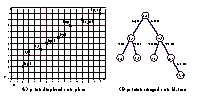
\includegraphics[scale=3]{img/kdt/dom-kd}
  \caption{Example of points indexed in a \kdtree{}.}
\end{figure}
\end{frame}

%
\begin{frame}
\frametitle{Multidimensional solution indexing}
Example of dominance check operation using \kdtree{}:
\begin{figure}
  \centering
  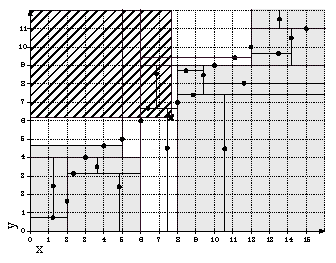
\includegraphics[scale=1.0]{img/kdt/query}
\end{figure}
\pause
The efficiency of this pruning action grows
with the amount of points.
\end{frame}


%
\begin{frame}
\frametitle{}
\begin{center}
  \textbf{\Large Multi-dimensional Indexing of MOKP solutions}
  \\ \bigskip \bigskip
  {\large Use case on an exact method}
\end{center}
\end{frame}

%
\begin{frame}
\frametitle{Nemhauser and Ullmann's algorithm}
As an application of the indexing proposal we will use the \kdtree{}
in an \textit{state-of-art} exact dynamic programming algorithm for the MOKP.
\\ \bigskip \pause
The algorithm can be seen as a MOKP specialization of the classical
Nemhauser and Ullmann's algorithm for generically solving knapsack problems.
\\ \bigskip \pause
\begin{algorithmic}[1] % The number tells where the line numbering should start
    \Function{DP}{$\bsym{p}, \bsym{w}, W$} \pause
    \State $S^0 = \big\{\emptyset\big\}$ \pause
    \For{$k \gets 1, n$}
      \State $S_*^k = S^{k-1} \cup \{\sol{x} \cup k \:|\: \sol{x} \in S^{k-1}\}$
        \Comment{solutions extension} \pause
      \State $S^k = \{\sol{x} \:|\: \nexists \sol{a} \in S_*^k: \domk{a}{x} \}$
        \Comment{partial dominance filter}
    \EndFor \pause
  \State $P = \{\sol{x} \:|\: \nexists \sol{a} \in S^n: \dom{a}{x} \;|\; \weight{x} \leq W \}$
    \Comment{dominance/feasibility} \pause
  \State \Return $P$
  \EndFunction
\end{algorithmic}
\end{frame}

%
\begin{frame}
\frametitle{Bazgan's dynamic programming algorithm}
\begin{center}
\only<2>{\alert{Item reordering}}
\only<4>{\alert{Feasible extension}}
\only<5>{\alert{Defficiency avoidance}}
\only<6>{\alert{Unpromising elimination}}
\end{center}

\begin{algorithmic}[1]
  \Function{BazDP}{$\bsym{p}, \bsym{w}, W$}
    \State $\solSet^0 = \big\{\emptyset\big\}$ \pause
    \State $o_1, \ldots, o_n = \ord^{max}$ \pause
    \For{$k \gets 1, n$} \pause
      % Extension
      \State $\solSett^k = \big\{\sol{x} \cup \{o_k\} \;\big|\; \sol{x}
        \in \solSet^{k-1} \logicAnd \weight{x} + w_{o_k} \leq W \big\}$ \pause
      % Extension (cont.)
      \State $\phantom{\solSett^k = } \cup \big\{ \sol{x} \;\big|\; \sol{x} \in \solSet^{k-1} \logicAnd
        \weight{x} + w_{o_k} + \ldots + w_{o_n} > W \big\}$ \pause
      % Dominance filter
      \State $\solSet^k = \left\{\sol{x} \in \solSett^k \;\middle|\;
        (\nexists \sol{a} \in \solSett^k)\big[\domk{a}{x}
          \logicOr dom\big(lb(\sol{a}), ub(\sol{x})\big)\big] \right\}$ \pause
    \EndFor
    \State \Return $\solSet^n$
  \EndFunction
\end{algorithmic}
\end{frame}
% slide copy...
\begin{frame}
\frametitle{Bazgan's dynamic programming algorithm}
\begin{center}
\alert{Dominance check operation}
\end{center}
\begin{algorithmic}[1]
  \Function{BazDP}{$\bsym{p}, \bsym{w}, W$}
    \State $\solSet^0 = \big\{\emptyset\big\}$
    \State $o_1, \ldots, o_n = \ord^{max}$
    \For{$k \gets 1, n$}
      % Extension
      \State $\solSett^k = \big\{\sol{x} \cup \{o_k\} \;\big|\; \sol{x}
        \in \solSet^{k-1} \logicAnd \weight{x} + w_{o_k} \leq W \big\}$
      % Extension (cont.)
      \State $\phantom{\solSett^k = } \cup \big\{ \sol{x} \;\big|\; \sol{x} \in \solSet^{k-1} \logicAnd
        \weight{x} + w_{o_k} + \ldots + w_{o_n} > W \big\}$
      % Dominance filter
      \State $\solSet^k = \left\{\sol{x} \in \solSett^k \;\middle|\;
        (\nexists \sol{a} \in \solSett^k)\big[\alert{\underline{dom_k}}(\sol{a}, \sol{x})
          \logicOr \alert{\underline{dom}}\big(lb(\sol{a}), ub(\sol{x})\big)\big] \right\}$
    \EndFor
    \State \Return $\solSet^n$
  \EndFunction
\end{algorithmic}
\end{frame}

%
\begin{frame}
\frametitle{Computational Experiments}
Computational experiments on bi-dimensional instances:
\begin{enumerate}
  \item[A)]{ Random instances:\\
    $p^j_i \in [1, 1000]$,\\
    $w_i \in [1,1000]$.} \medskip
  \item[B)]{ Unconflicting instances: \\
    $p^1_i \in [111, 1000],$ \\
    $p^2_i \in [p^1_i - 100, p^1_i + 100],$ \\
    $w_i \in [1,1000]$.} \medskip
  \item[C)]{ Conflicting instances: \\
    $p^1_i \in [1, 1000],$ \\
    $p^2_i \in [max\{900-p^1_i;1\}, min\{1100-p^1_i, 1000\}],$ \\
    $w_i \in [1,1000]$.} \medskip
  \item[D)]{ Conflicting instances with correlated weight: \\
    $p^1_i \in [1, 1000],$ \\
    $p^2_i \in [max\{900-p^1_i;1\}, min\{1100-p^1_i, 1000\}],$ \\
    $w_i \in [p^1_i+p^2_i-200, p^1_i+p^2_i+200]$.}
\end{enumerate}
\end{frame}

%
\begin{frame}
\frametitle{Computational Experiments}
Average CPU-time for bi-objective instances:
\begin{table}[]
  \renewcommand*{\arraystretch}{0.9}
  \centering
  \begin{tabular}{crr|r|rr}
  \hline
  %%%%%%%%%%%%%%%%%
  %   HEADER
  %%%%%%%%%%%%%%%%%
  \multicolumn{3}{c|}{Instance}
  & AVL tree
  & \multicolumn{2}{c}{\dtree{2}}
    \\
  Type
  & $n$
  & $|ND| $
  & time (s)
  & time (s)
  & speedup
    \\ \hline
\multirow{2}{*}{A}
 &  40 &   38.1 & \textbf{0.06} & \textbf{  0.06} &  1.0 \\
 &  60 &   73.1 &    1.12 & \textbf{  0.88} &  1.3 \\
 &  80 &  125.6 &   19.81 & \textbf{ 11.89} &  1.7 \\
 & 100 &  180.4 &  165.24 & \textbf{ 76.50} &  2.2 \\
 & 120 &  233.9 &  708.53 & \textbf{361.87} &  2.0 \\ \hline
\multirow{2}{*}{B}
 & 100 &    3.1 & \textbf{  0.02} &    0.08 &  0.3 \\
 & 200 &   10.0 & \textbf{  0.80} &    5.09 &  0.2 \\
 & 300 &   24.9 & \textbf{  9.45} &   88.30 &  0.1 \\
 & 400 &   36.2 & \textbf{ 95.39} &  730.04 &  0.1 \\
 & 500 &   53.7 & \textbf{255.57} & 2824.65 &  0.1 \\
 \hline
\multirow{2}{*}{C}
 &  20 &   36.6 & \textbf{0.00} & \textbf{   0.00} &  1.0 \\
 &  40 &  102.8 &    0.65 & \textbf{   0.42} &  1.5 \\
 &  60 &  231.9 &   28.98 & \textbf{  14.09} &  2.1 \\
 &  80 &  358.0 &  564.10 & \textbf{ 241.54} &  2.3 \\
 & 100 &  513.8 & 3756.57 & \textbf{1605.19} &  2.3 \\ \hline
\multirow{2}{*}{D}
 &  20 &  174.9 &    0.15 & \textbf{   0.12} &  1.3 \\
 &  30 &  269.3 &   16.82 & \textbf{   7.60} &  2.2 \\
 &  40 &  478.0 &  395.76 & \textbf{ 186.67} &  2.1 \\
 &  50 &  553.4 & 2459.48 & \textbf{1417.94} &  1.7 \\ \hline
\end{tabular}

\end{table}
\end{frame}


%
\begin{frame}
\frametitle{Computational Experiments}
Average number of solution evaluations for bi-objective instances:
\begin{figure}
  \centering
\begin{subfigure}{.5\textwidth}
  \centering
  \begin{tikzpicture}
\begin{axis}[
	x tick label style={ /pgf/number format/1000 sep=},
	width=\cmpW, height=\cmpH,
	ylabel=Evaluations,
	ymode=log,
	grid = both,
	grid style={line width=.1pt, draw=gray!10},
	major grid style={line width=.2pt,draw=gray!50},
	%xlabel=Number of items (n),
	enlargelimits=0.15,
	legend style={at={(\legX,\legY)},
		anchor=north,legend columns=-1},
	ybar=2.6pt,% configures `bar shift'
	bar width=9pt,
	point meta=y *10^-7, % the displayed number
	cycle list = {black!80,black!30}
]

\addplot+[fill, text=black]
  coordinates {
    ( 40,3703070)
    ( 60,103534833)
    ( 80,700026931)
    (100,5542292786)
    (120,4935519921)
  };

\addplot+[fill, text=black]
  coordinates {
    ( 40,291655)
    ( 60,1182225)
    ( 80,5434379)
    (100,27996835)
    (120,31578018)
  };

\legend {AVL-tree,\dtree{2}}
\end{axis}
\end{tikzpicture}
  \caption{Type A}
  \label{fig:sub1}
\end{subfigure}%
\begin{subfigure}{.5\textwidth}
  \centering
  
\begin{tikzpicture}
\begin{axis}[
	x tick label style={ /pgf/number format/1000 sep=},
	width=\cmpW, height=\cmpH,
	ylabel=Avaliações,
	ymin=100000,
	ymax=100000000000,
	ymode=log,
	grid = both,
	grid style={line width=.1pt, draw=gray!10},
	major grid style={line width=.2pt,draw=gray!50},
	%xlabel=Number of items (n),
	enlargelimits=0.15,
	legend style={at={(\legX,\legY)},
		anchor=north,legend columns=-1},
	ybar=2pt,% configures `bar shift'
	bar width=8pt,
	xtick={100,200,300,400,500},
	xticklabels={100,200,300,400,500},
	point meta=y *10^-7, % the displayed number
	cycle list = {black!80,black!30}
]

\addplot+[fill, text=black]
  coordinates {
    (100,562886)
    (200,27327963)
    (300,349249789)
    (400,17406619609)
    (500,12137619611)
  };

\addplot+[fill, text=black]
  coordinates {
    (100,330881)
    (200,5329798)
    (300,396002213)
    (400,148865700)
    (500,318904809)
  };

\legend {AVL-tree,\dtree{2}}
\end{axis}
\end{tikzpicture}

  \caption{Type B}
  \label{fig:sub2}
\end{subfigure}
\begin{subfigure}{.5\textwidth}
  \centering
  
\begin{tikzpicture}
\begin{axis}[
	x tick label style={ /pgf/number format/1000 sep=},
	width=\cmpW, height=\cmpH,
	ylabel=Avaliações,
	ymin=100000,
	ymax=100000000000,
	ymode=log,
	grid = both,
	grid style={line width=.1pt, draw=gray!10},
	major grid style={line width=.2pt,draw=gray!50},
	%xlabel=Number of items (n),
	enlargelimits=0.15,
	legend style={at={(\legX,\legY)},
		anchor=north,legend columns=-1},
	ybar=2pt,% configures `bar shift'
	bar width=9pt,
	point meta=y *10^-7, % the displayed number
	cycle list = {black!80,black!30}
]

\addplot+[fill, text=black]
  coordinates {
    ( 20,191729)
    ( 40,18662815)
    ( 60,670819408)
    ( 80,4616460680)
    (100,73868244070)
  };

\addplot+[fill, text=black]
  coordinates {
    ( 20,32950)
    ( 40,926315)
    ( 60,5542258)
    ( 80,23285877)
    (100,80371740)
  };

\legend {AVL-tree,\dtree{2}}
\end{axis}
\end{tikzpicture}

  \caption{Type C}
  \label{fig:sub3}
\end{subfigure}%
\begin{subfigure}{.5\textwidth}
  \centering
  
\begin{tikzpicture}
\begin{axis}[
	x tick label style={ /pgf/number format/1000 sep=},
	width=\cmpW, height=\cmpH,
	ylabel=Avaliações,
	ymin=100000,
	ymax=100000000000,
	ymode=log,
	grid = both,
	grid style={line width=1.3pt, draw=gray!00},
	major grid style={line width=.2pt,draw=gray!50},
	%xlabel=Number of items (n),
	enlargelimits=0.15,
	legend style={at={(\legX,\legY)},
		anchor=north,legend columns=-1},
	ybar=2pt,% configures `bar shift'
	xmin=18,
	xmax=52,
	bar width=9pt,
	point meta=y *10^-7, % the displayed number
	cycle list = {black!80,black!30}
]

\addplot+[fill, text=black]
  coordinates {
    ( 20,2831448)
    ( 30,489772231)
    ( 40,9316773179)
    ( 50,19581372744)
  };

\addplot+[fill, text=black]
  coordinates {
    ( 20,173245)
    ( 30,3317384)
    ( 40,14262798)
    ( 50,57959241)
  };

\legend {AVL-tree,\dtree{2}}
\end{axis}
\end{tikzpicture}

  \caption{Type D}
  \label{fig:sub4}
\end{subfigure}
\end{figure}
\end{frame}

%
\begin{frame}
\frametitle{Computational Experiments}
Average CPU-time for 3-objective instances:
\begin{table}[]
  \renewcommand*{\arraystretch}{0.9}
  \centering
  \begin{tabular}{crr|r|rc|rc}
  \hline
  %%%%%%%%%%%%%%%%%
  %   HEADER
  %%%%%%%%%%%%%%%%%
  \multicolumn{3}{c|}{Instance}
  & AVL tree
  & \multicolumn{2}{c|}{\dtree{2}}
  & \multicolumn{2}{c}{\dtree{3}}
    \\
  Type
  & $n$
  & $|ND| $
  & time (s)
  & time (s)
  & speedup
  & time (s)
  & speedup
    \\ \hline
  %%%%%%%%%%%%%%%%%
  %   CLASS A
  %%%%%%%%%%%%%%%%%
  \multirow{2}{*}{A}
  & 50 &  557.5 &    41.2 &    21.3 & 1.9 & \textbf{  18.5} & 2.2 \\
  & 60 & 1240.0 &   485.9 &   247.8 & 1.9 & \textbf{  79.9} & 6.0 \\
  & 70 & 1879.3 &  3179.5 &  1038.0 & 3.0 & \textbf{ 614.5} & 5.1 \\
  & 80 & 2540.5 &  6667.9 &  3796.0 & 1.7 & \textbf{2943.9} & 2.2 \\
  & 90 & 3528.5 & 24476.5 & 12916.7 & 1.8 & \textbf{3683.7} & 6.6 \\ \hline
  %%%%%%%%%%%%%%%%
  %   CLASS B
  %%%%%%%%%%%%%%%%%
  \multirow{2}{*}{B}
  & 100 &  18.0 & \textbf{   0.1} &    0.3 & 0.3 &    0.3 & 0.3 \\
  & 200 &  65.4 & \textbf{  11.4} &   34.4 & 0.3 &   29.1 & 0.4 \\
  & 300 & 214.2 & \textbf{ 307.7} &  631.5 & 0.5 &  583.2 & 0.5 \\
  & 400 & 317.0 & \textbf{4492.9} & 8464.9 & 0.5 & 5402.2 & 0.8 \\ \hline
  %%%%%%%%%%%%%%%%%
  %   CLASS C
  %%%%%%%%%%%%%%%%%
  \multirow{2}{*}{C}
  & 20 &  254.4 &   0.06 &   0.05 & 1.2 & \textbf{ 0.03} & 2.17 \\
  & 30 & 1066.6 &   9.69 &   4.18 & 2.3 & \textbf{ 1.30} & 7.46 \\
  & 40 & 2965.5 & 471.68 & 153.21 & 3.1 & \textbf{30.50} & 15.5 \\ \hline
  %%%%%%%%%%%%%%%%
  %   CLASS D
  %%%%%%%%%%%%%%%%%
  \multirow{2}{*}{D}
  & 20 & 4087.7 &   23.6 &   10.9 & 2.2 & \textbf{   1.9} & 12.5 \\
  & 30 & 8834.5 & 8914.2 & 3625.3 & 2.5 & \textbf{1019.5} &  8.7 \\ \hline
\end{tabular}
\end{table}
\end{frame}


%
\begin{frame}
\frametitle{Computational Experiments}
Average number of solution evaluations for 3-objective instances:
\begin{figure}
  \centering
\begin{subfigure}{.5\textwidth}
  \centering
  %\begin{tikzpicture}
\begin{axis}[
	x tick label style={ /pgf/number format/1000 sep=},
	width=\cmpW, height=\cmpH,
	ylabel=Avaliações,
	ymode=log,
	grid = both,
	grid style={line width=.0pt, draw=gray!00},
	major grid style={line width=.2pt,draw=gray!50},
	%xlabel=Number of items (n),
	enlargelimits=0.15,
	legend style={at={(\legX,\legY)},
		anchor=north,legend columns=-1},
	ybar=2pt,% configures `bar shift'
	bar width=7pt,
	point meta=y *10^-7, % the displayed number
	cycle list = {black!80,black!50,black!20}
]

\addplot+[fill, text=black]
  coordinates {
    (50,2557230768)
    (60,1548431035)
    (70,22725915563)
    (80,105604506342)
    (90,243276893280)
  };

\addplot+[fill, text=black]
  coordinates {
    (50,116409692)
    (60,2490816101)
    (70,6444320225)
    (80,40077812473)
    (90,84001331660)
  };
  
\addplot+[fill, text=black]
  coordinates {
    (50,6441918)
    (60,11026583)
    (70,42167703)
    (80,71599151)
    (90,174737779)
  };

\legend {AVL-tree,\dtree{2}, \dtree{3}}
\end{axis}
\end{tikzpicture}

  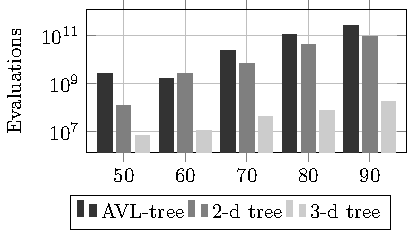
\includegraphics[scale=1.1]{tab/cmp/3dimA}
  \caption{Tipo A}
  \label{fig:sub5}
\end{subfigure}%
\begin{subfigure}{.5\textwidth}
  \centering
  %\begin{tikzpicture}
\begin{axis}[
	x tick label style={ /pgf/number format/1000 sep=},
	width=\cmpW, height=\cmpH,
	ylabel=Evaluations,
	ymode=log,
	grid = both,
	grid style={line width=.0pt, draw=gray!00},
	major grid style={line width=.2pt,draw=gray!50},
	%xlabel=Number of items (n),
	enlargelimits=0.15,
	legend style={at={(\legX,\legY)},
		anchor=north,legend columns=-1},
	ybar=2pt,% configures `bar shift'
	bar width=7pt,
	point meta=y *10^-7, % the displayed number
	cycle list = {black!80,black!50,black!20}
]

\addplot+[fill, text=black]
  coordinates {
    (100,2580591.4)
    (200,367842367.9)
    (300,7975491375.7)
    (400,72030125537.7)
  };

\addplot+[fill, text=black]
  coordinates {
    (100,1571248.6)
    (200,151476739.2)
    (300,2791493175.3)
    (400,45272872459.5)
  };
  
\addplot+[fill, text=black]
  coordinates {
    (100,912878.0)
    (200,29237583.4)
    (300,226471349.8)
    (400,960366212.0)
  };

\legend {AVL-tree,\dtree{2}, \dtree{3}}
\end{axis}
\end{tikzpicture}
  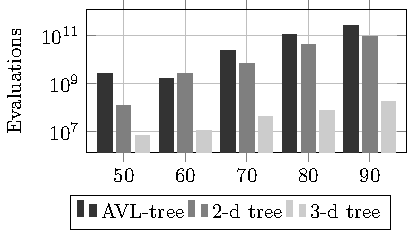
\includegraphics[scale=1.1]{tab/cmp/3dimA}
  \caption{Tipo B}
  \label{fig:sub6}
\end{subfigure}
\begin{subfigure}{.49\textwidth}
  \centering
  %\begin{tikzpicture}
\begin{axis}[
	x tick label style={ /pgf/number format/1000 sep=},
	width=\cmpW, height=\cmpH,
	ylabel=Avaliações,
	ymode=log,
	grid = both,
	grid style={line width=.1pt, draw=gray!00},
	major grid style={line width=.2pt,draw=gray!50},
	%xlabel=Number of items (n),
	enlargelimits=0.15,
	xtick={20, 30, 40},
	xticklabels={20, 30, 40},
	xmin=18,
	xmax=42,
	legend style={at={(\legX,\legY)},
		anchor=north,legend columns=-1},
	ybar=2pt,% configures `bar shift'
	bar width=7pt,
	point meta=y *10^-7, % the displayed number
	cycle list = {black!80,black!50,black!20}
]

\addplot+[fill, text=black]
  coordinates {
    ( 20,221956989)
    ( 30,10861341339)
    ( 40,26505319423)
  };

\addplot+[fill, text=black]
  coordinates {
    ( 20,235426288)
    ( 30,1340276850)
    ( 40,5943925097)
  };
  
\addplot+[fill, text=black]
  coordinates {
    ( 20,1919561)
    ( 30,10225751)
    ( 40,63529280)
  };

\legend {AVL-tree,\dtree{2}, \dtree{3}}
\end{axis}
\end{tikzpicture}

  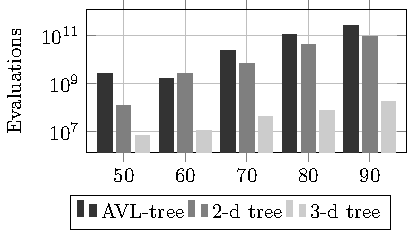
\includegraphics[scale=1.1]{tab/cmp/3dimA}
  \caption{Tipo C}
  \label{fig:sub7}
\end{subfigure}
\begin{subfigure}{.49\textwidth}
  \centering
  %\begin{tikzpicture}
\begin{axis}[
	x tick label style={ /pgf/number format/1000 sep=},
	width=\cmpW, height=\cmpH,
	ylabel=Evaluations,
	ymode=log,
	grid = both,
	grid style={line width=.0pt, draw=gray!00},
	major grid style={line width=.2pt,draw=gray!50},
	%xlabel=Number of items (n),
	enlargelimits=0.15,
	xtick={20, 30},
	xmin=17,
	xmax=33,
	legend style={at={(\legX,\legY)},
		anchor=north,legend columns=-1},
	ybar=2pt,% configures `bar shift'
	bar width=8pt,
	point meta=y *10^-7, % the displayed number
	cycle list = {black!80,black!50,black!20}
]

\addplot+[fill, text=black]
  coordinates {
    (20,481435295.3)
    (30,89269703684.8)
  };

\addplot+[fill, text=black]
  coordinates {
    (20,161607530.0)
    (30,32867842298.12)
  };
  
\addplot+[fill, text=black]
  coordinates {
    (20,2127432.7)
    (30,59136651.9)
  };

\legend {AVL-tree,\dtree{2}, \dtree{3}}
\end{axis}
\end{tikzpicture}
  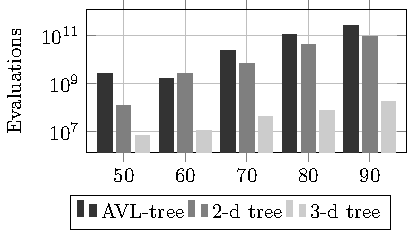
\includegraphics[scale=1.1]{tab/cmp/3dimA}
  \caption{Tipo D}
  \label{fig:sub8}
\end{subfigure}

\end{figure}
\end{frame}


%
\begin{frame}
\frametitle{Conclusions}
The multi-dimensional indexing is applicable to the problem requiring
considerably less solution evaluations, especially on hard instances.
\\ \medskip \pause
Algorithm speedup $2.3$ for bi-dimensional
cases and up to $15.5$ on 3-dimensional cases.
\\ \medskip \pause
The multi-dimensional indexing was not efficient on \textit{easy} instances
for which the set of solutions is relatively small.
\\ \medskip \pause
Several instances are still intractable due
the large number of intermediate solutions.
\\ \medskip \pause
For this reason this work proposes to use the indexing strategy
in conjunction with an evolutionary metaheuristic.
\end{frame}
